\documentclass[10pt]{beamer}

\usetheme[progressbar=frametitle]{metropolis}
\definecolor{ag-maroon}{RGB}{80,0,0}
\definecolor{ag-maroon2}{RGB}{60,0,0}
\definecolor{ag-blue}{RGB}{0,60,113}
\definecolor{ag-odgreen}{RGB}{91,98,54}
\definecolor{ag-brown}{RGB}{116,79,40}
\definecolor{ag-tan}{RGB}{153,133,66}
\definecolor{ag-beige}{RGB}{214,210,196}
\definecolor{ag-white}{RGB}{246,246,246}
\definecolor{ag-black}{RGB}{0,0,0}
\definecolor{ag-light-black}{RGB}{20,20,20}

\setbeamercolor{background canvas}{fg=ag-white}
\setbeamercolor{normal text}{fg=ag-black}
\setbeamercolor{alerted text}{fg=ag-tan}
\setbeamercolor{example text}{fg=ag-light-black}

\setbeamercolor{frametitle}{bg=ag-blue}
\setbeamercolor{progress bar}{fg=ag-maroon}
\setbeamercolor{title separator}{fg=ag-blue}
\setbeamercolor{progress bar in head/foot}{fg=ag-tan}
\setbeamercolor{progress bar in section page}{fg=ag-tan}


\usepackage{appendixnumberbeamer}

\usepackage{booktabs}
\usepackage[scale=2]{ccicons}

\usepackage{pgfplots}
\usepgfplotslibrary{dateplot}

\usepackage{xspace}
\newcommand{\themename}{\textbf{\textsc{metropolis}}\xspace}

\usepackage{amsfonts,amsmath,amssymb,amsthm}
\usepackage{graphicx}
\graphicspath{{../figures}}
\usepackage{tikz}
\usetikzlibrary{positioning}

\usepackage{tcolorbox}
\usepackage{multirow}
\usepackage{subcaption}

%%%%%%%%%%%%%%%%%%%
% Custom commands

\newcommand{\bb}[1]{\boldsymbol{#1}}
\newcommand{\tr}{^{\intercal}}
\newcommand{\R}{\mathbb{R}}
\newcommand{\E}{\mathbb{E}}
\newcommand{\argmax}{\arg\,\max}

%%%%%%%%%%%%%%%%%%
% TITLE AREA
\title{Robust Principal Component Analysis using Density Power Divergence}
% \subtitle{A Robust Singular Value Decomposition Technique}
% \date{\today}
\date{}
\author{Subhrajyoty Roy}
\institute{Research Fellow, Interdisciplinary Statistical Research Unit\\
    Indian Statistical Institute, Kolkata, India\\
    \textbf{Supervisors:} Ayanendranath Basu \& Abhik Ghosh
    \begin{flushright}
        Dec, 2024,\\
        IISA Conference
    \end{flushright}
}
% \titlegraphic{\hfill
\includegraphics[height=1.5cm]{logo.pdf}}


\makeatletter
\let\save@measuring@true\measuring@true
\def\measuring@true{%
  \save@measuring@true
  \def\beamer@sortzero##1{\beamer@ifnextcharospec{\beamer@sortzeroread{##1}}{}}%
  \def\beamer@sortzeroread##1<##2>{}%
  \def\beamer@finalnospec{}%
}
\makeatother

\begin{document}

\maketitle

\begin{frame}{Principal Component Analysis (PCA)}
    
    \begin{tcolorbox}[colback=green!5!white,colframe=green!75!black]

    Given an independent and identically distributed sample $X_1, X_2, \dots X_n$, each $X_i \in \R^p$, and a scale measure $S_n(y_1, \dots y_n)$, first principal component is 
    \begin{equation*}
        \widehat{\bb{v}}_1 = \argmax_{\bb{v} \in \R^p, \Vert v\Vert = 1} S_n(\bb{v}\tr X_1, \bb{v}\tr X_2, \dots, \bb{v}\tr X_n),
    \end{equation*}
    \noindent and the eigenvalue is 
    \begin{equation*}
        \widehat{\lambda}_1 = S_n(\widehat{\bb{v}}_1\tr X_1, \widehat{\bb{v}}_1\tr X_2, \dots, \widehat{\bb{v}}_1\tr X_n).
    \end{equation*}
    \noindent Subsequent principal components are defined similarly subject to orthogonality conditions.
    \end{tcolorbox}
    
\end{frame}

\begin{frame}{Effect of outlier on PCA}
    \begin{figure}
        \centering
        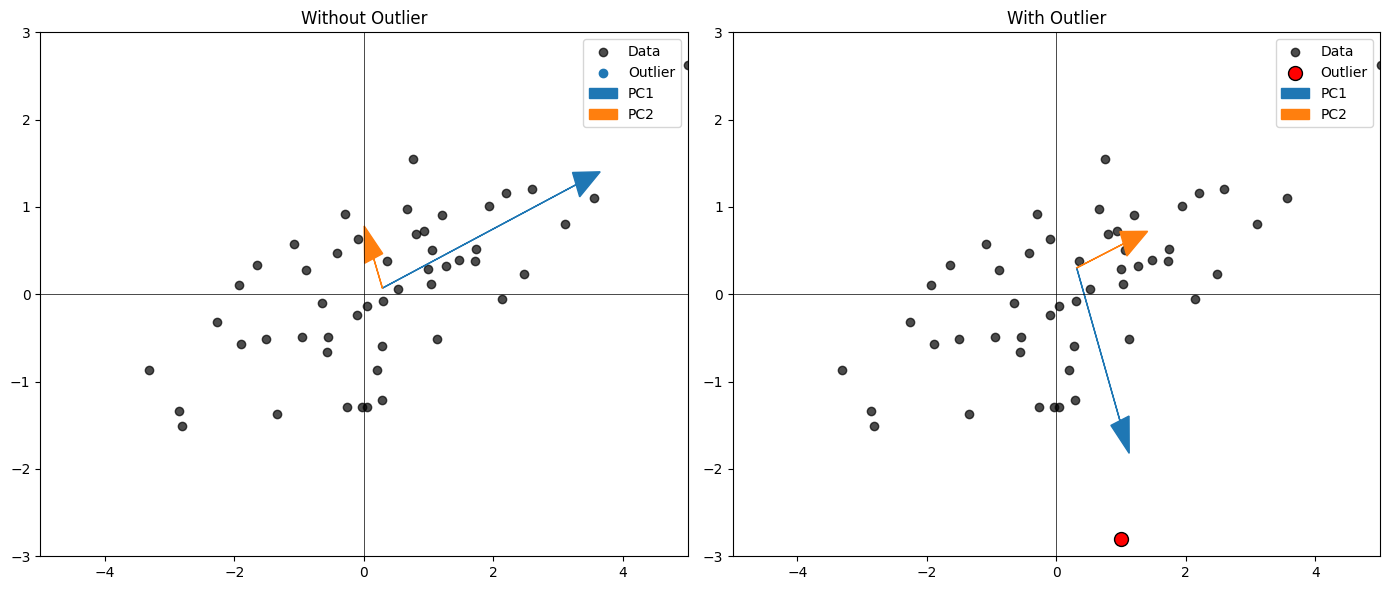
\includegraphics[width = \textwidth]{figures/thesis_slides/outlier-with-without.png}
        \caption{Data generated from multivariate normal. A single outlier can greatly distort the principal component eigenvalues and eigenvectors.}
    \end{figure}
\end{frame}

\begin{frame}{Alternative formulation of PCA}
    Consider, 
    \begin{equation*}
        \bb{X} = \begin{bmatrix}
            X_1\tr \\ X_2\tr \\ \vdots \\ X_n\tr
        \end{bmatrix}_{n \times p}
    \end{equation*}
    \noindent and if $S_n$ is the standard deviation, then 
    \begin{equation*}
        \dfrac{1}{n}\bb{X}\tr\bb{X} = \sum_{k=1}^{r} \lambda_k \bb{v}_k\bb{v}_k\tr + \bb{E}_1
    \end{equation*}
    \pause
    \noindent If we consider the same SVD decomposition
    \begin{equation*}
        \bb{X} = \bb{UDV}\tr + \bb{E} = \bb{L} + \bb{E},
    \end{equation*}    
    \noindent with $\bb{D} = \text{Diag}(\sqrt{n\lambda_1}, \dots, \sqrt{n \lambda_p})$, and $\bb{L}$ is a low-rank matrix.
\end{frame}

\begin{frame}{PCA as alternating regression}
    \begin{align*}
     & \bb{X} = \bb{L} + \bb{E}, \text{ where, } \bb{E} = ((\epsilon_{ij}))_{i,j}; \ \epsilon_{ij} \sim (1-\delta) g + \delta h\\
    \pause
    \Rightarrow \quad 
        & X_{ij} = \sum_{k=1}^{r} \sqrt{n\lambda_k} u_{ki} v_{kj} + \epsilon_{ij}, \ \lambda_k \text{ is eigenvalue, } u_{ki}, v_{kj} \text{ are singular vectors } \\
    \pause 
    \Rightarrow \quad 
        & X_{ij} = \sum_{k=1}^{r} a_{ki} b_{kj} + \epsilon_{ij};
        \ \text{assume, } a_{ki} = (n\lambda_k)^{1/4} u_{ki}, b_{kj} = (n\lambda_k)^{1/4} v_{kj}\\
    \end{align*}
    \pause
    Fixing $j$ yields, 
    \begin{equation*}
        \begin{bmatrix}
            X_{1j}\\
            X_{2j}\\
            \vdots\\
            X_{nj}
        \end{bmatrix} = 
        \begin{bmatrix}
            a_{11} & \dots & a_{r1}\\
            \vdots & \ddots & \vdots\\
            a_{1n} & \dots & a_{rn}
        \end{bmatrix}_{n \times r}
        \begin{bmatrix}
            b_{1j}\\
            b_{2j}\\
            \vdots\\
            b_{rj}
        \end{bmatrix} + 
        \begin{bmatrix}
            \epsilon_{1j}\\
            \epsilon_{2j}\\
            \vdots \\
            \epsilon_{nj}
        \end{bmatrix}
    \end{equation*}
\end{frame}

\begin{frame}{PCA as alternating regression}
    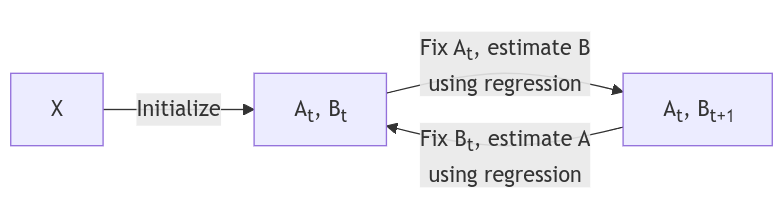
\includegraphics[width = \textwidth]{figures/thesis_slides/diagram.png}
    \begin{enumerate}
        \item \textbf{Scalable:} Avoids inversion of large matrices ($r << n, p$).
        \item \textbf{Fast and Parallelizable:} As each regression problem can be solved independently. 
    \end{enumerate}
    \pause
    \textbf{Note:} PCA is sensitive to outliers, since solving regression using \textbf{ordinary least squares} is sensitive to outliers.
\end{frame}

\begin{frame}{How to perform robust linear regression?}

    \begin{tcolorbox}[colback=green!5!white,colframe=green!75!black]
        \textbf{Density Power Divergence (DPD):} Given two density functions $f$ and $g$, \textcolor{blue}{Basu et al. (1998)} defines the DPD between them as
        \begin{equation*}
            d_\alpha(g, f) = \begin{cases}
                \displaystyle\int f^{1+\alpha} - \left(1+ \dfrac{1}{\alpha} \right)\displaystyle\int f^\alpha g + \dfrac{1}{\alpha} \displaystyle\int g^{1+\alpha}, & \alpha > 0\\
                \displaystyle\int f \log(f / g) & \alpha = 0
            \end{cases}
        \end{equation*}
    \end{tcolorbox}
    \pause
    \vspace*{0.5cm}
    Given an \textbf{independent but non-identically distributed} sample of observations $X_1, \dots X_n$ modelled by non-homogeneous families of densities $\{ f_{i,\theta}: \theta \in \Theta \}$, the \textbf{MDPDE} \textcolor{blue}{(Ghosh and Basu)} is defined as 
    \begin{equation*}
        \widehat{\theta}_\alpha = \arg\,\min_{\theta \in \Theta} \dfrac{1}{n}\sum_{i=1}^n \left[ \int f_{i, \theta}^{1+\alpha} - \left( 1 + \dfrac{1}{\alpha} \right) f_{i,\theta}^\alpha(X_i) \right], \ \alpha > 0.
    \end{equation*}
\end{frame}

\begin{frame}{Robust PCA using DPD}
    Assume estimation of the first principal component only,
    \begin{equation*}
        X_{ij} = a_i b_j + \epsilon_{ij}, \ \epsilon_{ij} \sim f(\cdot / \sigma), \sigma \in (0, \infty)
    \end{equation*}
    \noindent Assume form of $f$ is known and it is symmetric around $0$. 
    \pause 
    \begin{align*}
        & \textbf{Define weight function }\psi(\cdot)\\
        w_{ij}^{(t)} & = \psi\left( \vert X_{ij} - a_i^{(t)}b_{j}^{(t)} \vert / \sigma^{(t)}  \right), \ \psi(x) = -f^{\alpha-1}(\vert x\vert)f'(\vert x\vert) / \vert x\vert \\
        \pause
        & \textbf{Then, estimates are simply weighted averages as } x_{ij}/b_j \approx a_i \\
        a_i^{(t+1/2)} & = \left[ \sum_j (b_j^{(t)})^2 w_{ij}^{(t)} \right]^{-1} \left[ \sum_j (x_{ij} / b_j^{(t)}) (b_j^{(t)})^2 w_{ij}^{(t)} \right], \ i = 1, \ldots n; \\
        a_i^{(t+1)} & = a_i^{(t + 1/2)} / \Vert \bb{a}^{(t + 1/2)} \Vert, \ \text{ as we want unitary matrices} 
    \end{align*}
\end{frame}

\begin{frame}{Different choices of model family}

{
    \textbf{All the weight functions are decreasing!}\\
    \textbf{So more errors $\implies$ less weights.}
}

\begin{table}
    \centering
    \begin{tabular}{lrr}
        \toprule
        \textbf{Density family} & $\propto f(x)$ & $\psi(x)$ \\
        \midrule
         Normal & $e^{-x^2/2}$ & $e^{-\alpha x^2/2}$ \\
         Laplace & $e^{-\vert x\vert}$ & $e^{-\alpha\vert x\vert}/\vert x\vert$ \\
         $t_\nu$ & $(1+x^2/\nu)^{-(1+\nu)/2}$ & $(1 + 1/\nu)(1 + x^2/\nu)^{-\alpha(\nu + 1)/2 - 1}$\\
         Logistic & $e^{-x}/(1+e^{-x})^2$ & $e^{-\alpha x}(1 - e^{-x})/x(1+e^{-x})^{2\alpha + 1}$\\
         \bottomrule
    \end{tabular}
    \caption{The choices of $\psi(\cdot)$ functions for different elliptically symmetric family of densities.}
    \label{tab:rpca-psi-and-g}
\end{table}
\end{frame}



\begin{frame}{Results on rPCAdpd (Roy, Basu and Ghosh, 2024)}
    \noindent We assume $X_1, \dots X_n$ are from an elliptically symmetric density family,
    \begin{equation*}
        f_{\bb{\theta}}(\bb{x}) \propto \det(\bb{\Sigma})^{-1/2} \exp\left[ g\left( (\bb{x} - \bb{\mu})\tr \sum_{k=1}^p \gamma_k^{-1}\bb{v}_k\bb{v}_k\tr (\bb{x} - \bb{\mu}) \right) \right]
    \end{equation*}
    
    \begin{tcolorbox}[colback=green!5!white,colframe=green!75!black]
        If $g$ is decreasing and twice differentiable, the minimizer of DPD exists and the rPCAdpd algorithm converges.
    \end{tcolorbox}

    \begin{tcolorbox}[colback=green!5!white,colframe=green!75!black]
        If the mean $\widehat{\mu}$ is orthogonally equivariant, then the rPCAdpd estimates are orthogonally equivariant.
    \end{tcolorbox}
\end{frame}

\begin{frame}{Results on rPCAdpd (Roy, Basu and Ghosh, 2023)}
Typical consistency and asymptotic normality results with one caveat.

{
    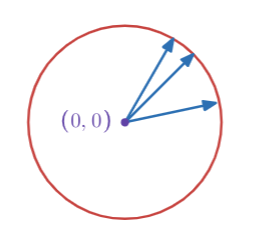
\includegraphics[width = 0.38\textwidth]{figures/thesis_slides/circle-eigen.png}
    \hfill
    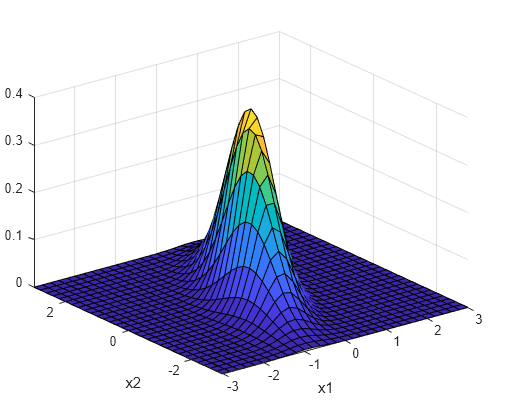
\includegraphics[width = 0.45\textwidth]{figures/thesis_slides/normal-eigen.png}
}

\pause

\begin{tcolorbox}[colback=green!5!white,colframe=green!75!black]
    If the true eigenvalues are distinct, then for any $n^c$-consistent mean estimator $\widehat{\mu}$ ($c \geq 1/2$), the rPCAdpd estimates of eigenvalues and \textbf{a natural parameter $\eta$ for the eigenvectors} are $\sqrt{n}$-consistent and are jointly asymptotically normal.
\end{tcolorbox}

\end{frame}



\begin{frame}{rPCAdpd for Gaussian case (Roy, Basu and Ghosh, 2023)}
    If $X_1, \dots, X_n$ are modelled using $p$-variate Gaussian family. Then for any $n^c$-consistent mean estimator $\widehat{\mu}$ ($c \geq 1/2$),
    \begin{enumerate}
        \item The estimated eigenvalues $\{ \widehat{\gamma}_k \}_{k=1}^p$ and the estimated eigenvectors $\{ \widehat{v}_k \}_{k=1}^p$ are asymptotically independent.
        \item $\sqrt{n}(\widehat{\bb{\gamma}} - \bb{\gamma})$ is asymptotically $p$-variate normally distributed with mean $\bb{0}$ and variance 
        \begin{equation*}
            \dfrac{(1+\alpha)^{p+4}}{(1+2\alpha)^{p/2}} \bb{M}^{-1} \left( A_\alpha \bb{J}_\gamma + \dfrac{1}{2(1+2\alpha)^2}\text{Diag}(\bb{\gamma})^{-2}  \right)\bb{M}^{-1}
        \end{equation*}
        \noindent where
        \begin{align*}
            J_\gamma & = (\text{Diag}(\gamma)^{-1})(\text{Diag}(\gamma)^{-1})\tr \\
            \bb{M} & = \left( \dfrac{\alpha^2}{4}J_\gamma + \dfrac{1}{2}\text{Diag}(\bb{\gamma})^{-2}  \right)\\
            A_\alpha & = \alpha^2 \left[ \dfrac{1}{(1+2\alpha)^2} - \dfrac{(1+2\alpha)^{p/2}}{4(1+\alpha)^{p+2}} \right]
        \end{align*}
    \end{enumerate}
\end{frame}

\begin{frame}{rPCAdpd for Gaussian case (Roy, Basu and Ghosh, 2023)}
    If $X_1, \dots, X_n$ are modelled using $p$-variate Gaussian family. Then for any $n^c$-consistent mean estimator $\widehat{\mu}$ ($c \geq 1/2$),
    \begin{enumerate}
        \setcounter{enumi}{2}
        \item For the natural parameter $\sqrt{n}(\widehat{\bb{\eta}} - \bb{\eta})$ is asymptotically $p$-variate normally distributed with $0$ and a variance 
        \begin{equation*}
            \dfrac{(1+\alpha)^{p/4}}{(1+2\alpha)^{2 + p/2}} \sum_{k,l} \left( 1 - \dfrac{\gamma_k}{\gamma_l} \right) \dfrac{\partial v_k}{\partial \bb{\eta}} v_k v_l\tr \left( \dfrac{\partial v_l}{\partial \bb{\eta}} \right)\tr
        \end{equation*}
    \end{enumerate}
\end{frame}

\begin{frame}{Additional Results}
    \begin{itemize}
        \item The estimator has a bounded influence function, if $\widehat{\mu}$ has bounded influence.
        \item The rPCAdpd estimator has asymptotic breakdown point at least $\alpha/(1+\alpha)$ which is free of $p$.
        \item Extensive simulation studies have been performed and compared against existing methods (PCP, spherical PCA, ROBPCA, projection pursuit- based methods, Geometric median-based PCA, etc.).
        \begin{itemize}
            \item Multiple levels of contaminations from $5\%$ to $20\%$.
            \item Cauchy and $t_5$ distribution of errors.
            \item Dimensions ranging from $p = 10$ to $p = 250$, with $n = 50$.
        \end{itemize}
        \item rPCAdpd beat existing methods even when $n < p$.
        \item Several benchmark datasets have been analyzed.
    \end{itemize}
\end{frame}

\begin{frame}{Simulation Results}
    \begin{table}[htbp]
        \caption{Estimated Bias and Mean Absolute Error of eigenvalues and Subspace Recovery Error of eigenvectors for different PCA algorithms (with $n = 50$).}
        \label{tbl:rpca-sim-S2b}
        \resizebox*{\textwidth}{!}{
        \begin{tabular}{ccrrrrrrrrrrrr}
            \toprule
            Metric & $p$ & Classical & LOC   & ROBPCA & Proj  & RobCov & Grid  & Gmed  & PCP   & \begin{tabular}[c]{@{}r@{}}DPD\\ (0.25)\end{tabular} & \begin{tabular}[c]{@{}r@{}}DPD\\ (0.5)\end{tabular} & \begin{tabular}[c]{@{}r@{}}DPD\\ (0.75)\end{tabular} & \begin{tabular}[c]{@{}r@{}}DPD\\ (1)\end{tabular} \\ \midrule
            \multirow{5}{*}{ Bias } & 10  & 0.321 & 0.757 & 0.381 & 0.429 & 0.589 & 0.757 & 0.14 & 1.065 & 0.329 & 0.281 & 0.138 & 0.067\\ 
            & 25  & 0.553 & 2.198 & 0.368 & 0.635 & 1.004 & 1.344 & 0.235 & 2.451 & 0.568 & 0.364 & 0.073 & 0.036\\ 
            & 50  & 1.467 & 4.602 & 0.829 & 1.796 & NA & 3.221 & 0.583 & 4.617 & 1.48 & 0.97 & 0.323 & 0.182\\ 
            & 100  & 2.66 & 9.414 & 1.028 & 2.692 & NA & 6.019 & 1.235 & 9.159 & 2.766 & 2.005 & 0.533 & 0.2\\ 
            & 250  & 7.033 & 23.805 & 3.245 & 8.006 & NA & 15.969 & 2.746 & 22.799 & 7.089 & 4.447 & 1.446 & 0.299\\ 
            \midrule
            \multirow{5}{*}{ MAE } & 10  & 41.99 & 75.693 & 43.08 & 52.712 & 60.646 & 82.448 & 30.185 & 106.511 & 45.196 & 42.803 & 29.261 & 22.409\\ 
            & 25  & 85.197 & 219.781 & 63.246 & 93.376 & 112.498 & 165.495 & 65.545 & 245.114 & 90.83 & 74.713 & 45.453 & 41.413\\ 
            & 50  & 194.589 & 460.223 & 130.581 & 236.929 & NA & 406.956 & 144.635 & 462.199 & 209.841 & 172.386 & 110.373 & 96.321\\ 
            & 100  & 364.678 & 941.397 & 221.517 & 400.614 & NA & 665.195 & 267.786 & 916.897 & 394.475 & 317.498 & 173.981 & 142.885\\ 
            & 250  & 957.207 & 2380.505 & 618.404 & 1066.532 & NA & 1696.499 & 658.65 & 2283.607 & 1060.277 & 838.361 & 545.85 & 432.927\\
            \midrule 
            \multirow{5}{*}{SRE} & 10  & 1.812 & 2.049 & 1.109 & 2.346 & 1.424 & 2.886 & 1.889 & 1.197 & 1.811 & 1.774 & 1.405 & 1.111\\ 
            & 25  & 2.14 & 2.422 & 1.021 & 2.645 & 2.212 & 4.19 & 2.26 & 1.276 & 2.152 & 1.832 & 1.111 & 1.03\\ 
            & 50  & 2.219 & 2.472 & 1.02 & 2.828 & NA & 4.985 & 2.314 & 2.265 & 2.24 & 1.819 & 1.201 & 1.049\\ 
            & 100  & 2.227 & 2.453 & 1.043 & 2.868 & NA & 3.86 & 2.326 & 2.272 & 2.242 & 1.868 & 1.153 & 1.007\\ 
            & 250  & 2.249 & 2.549 & 1.066 & 2.976 & NA & 3.901 & 2.362 & 2.302 & 2.262 & 1.767 & 1.16 & 1.007\\ 
            \bottomrule
        \end{tabular}}
    \end{table}
\end{frame}

\begin{frame}{Credit Card Fraud Detection Data Analysis}

{
    \small $28$ anonymized features with $n = 284807$ transactions, with $<0.1\%$ being frauds. We take first $5$ principal components, explaining over $80\%$ of variation.
}

\begin{columns}
    \column{0.35\textwidth}{
        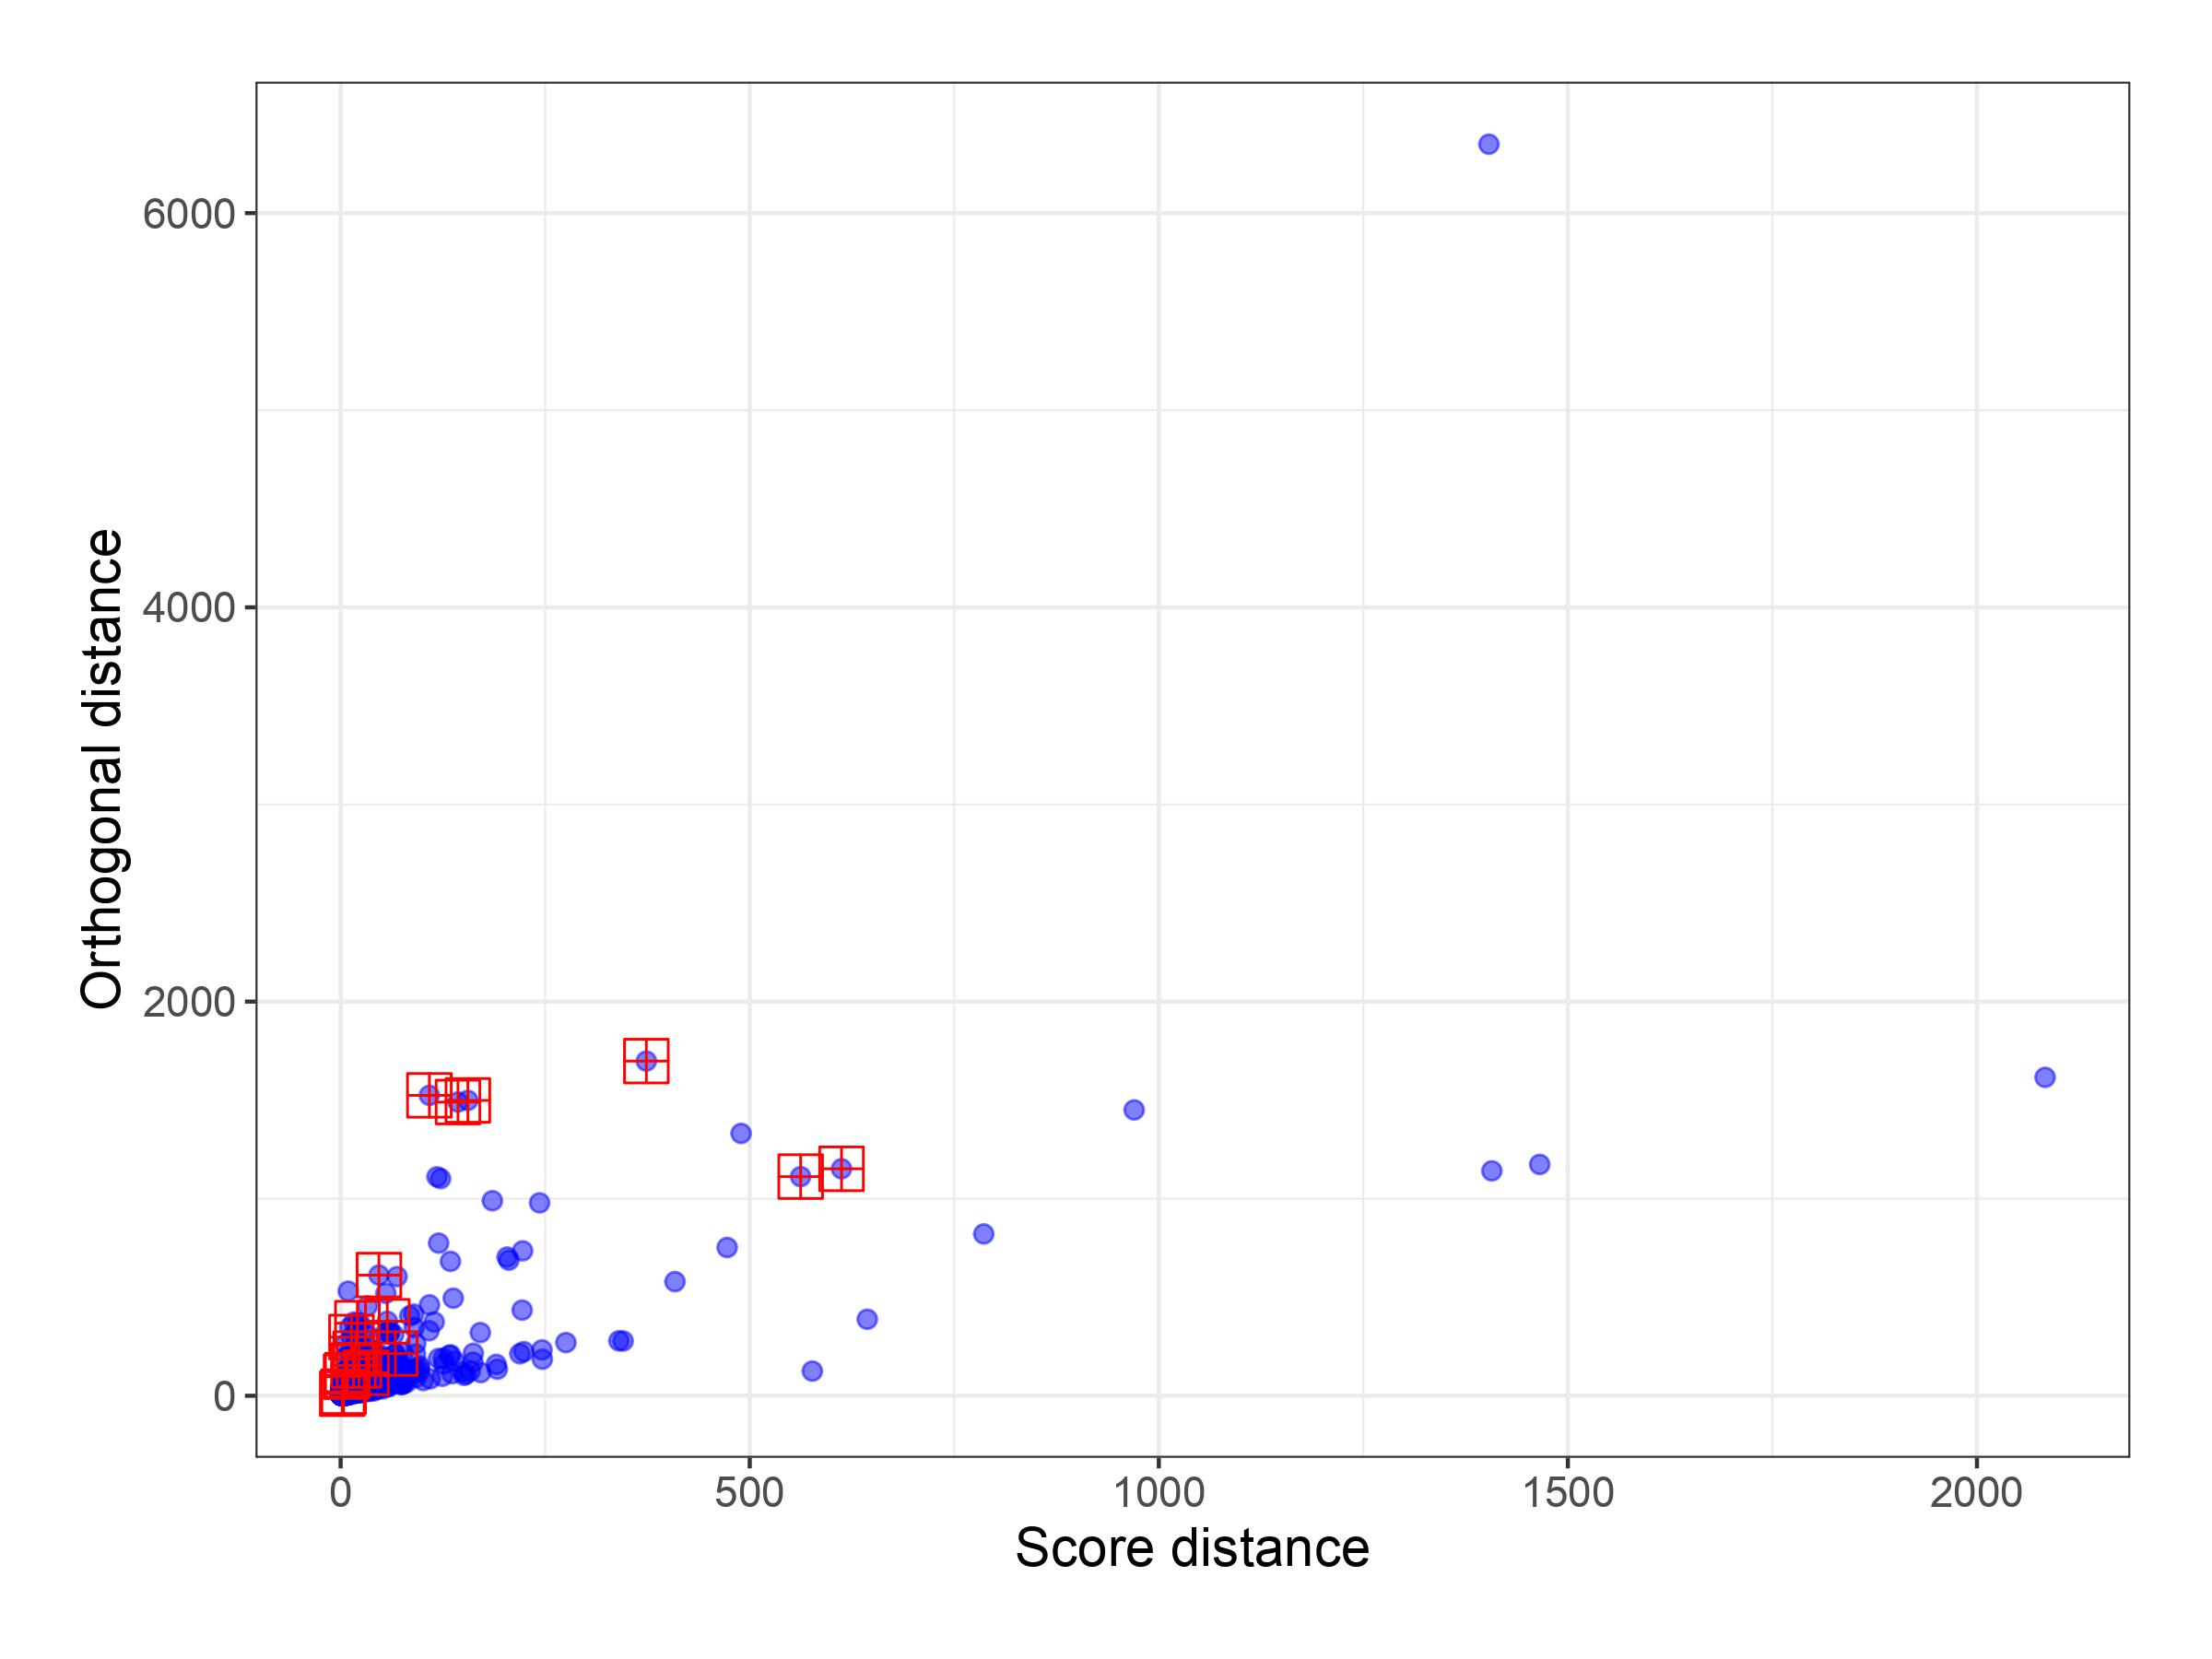
\includegraphics[width=\textwidth]{figures/rpcadpd/CCard-Classical.jpg}
        {\tiny (a) Classical PCA}
        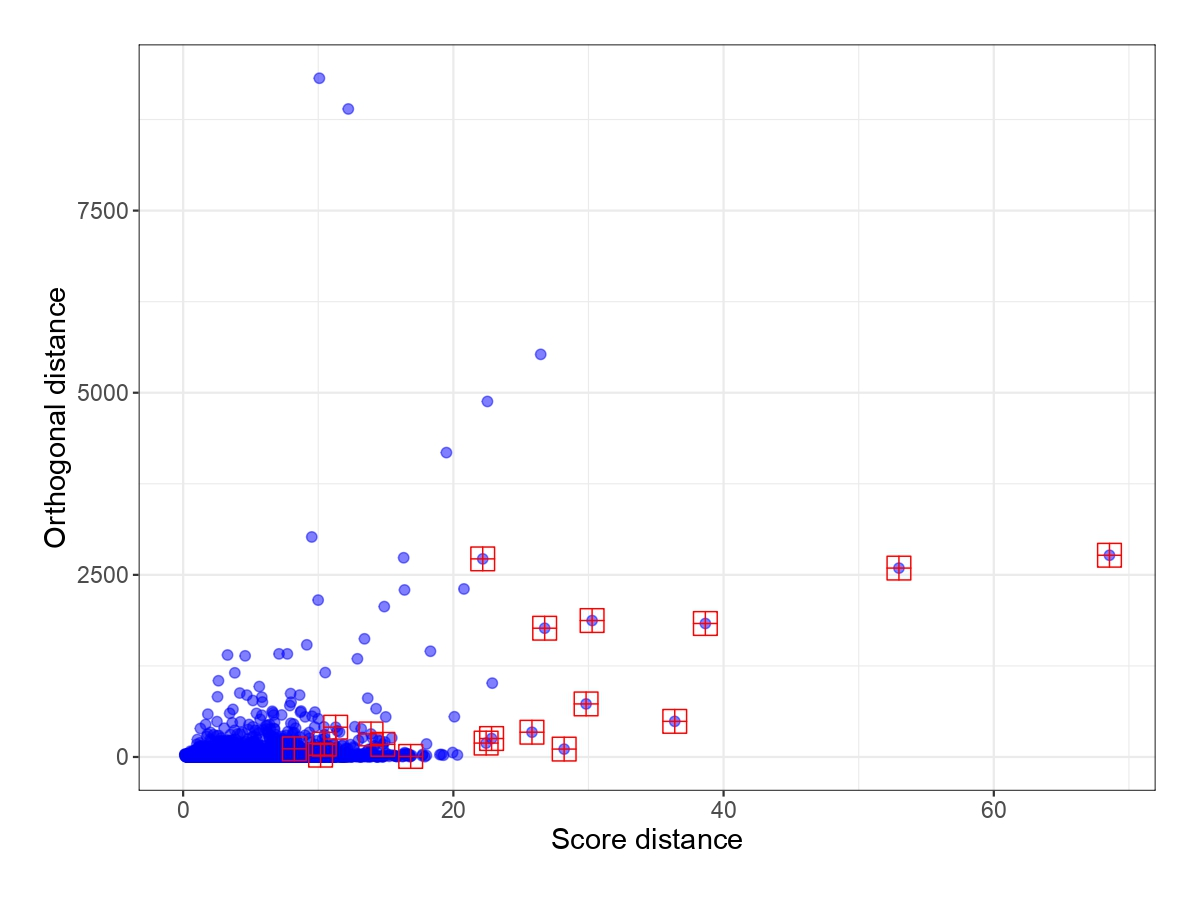
\includegraphics[width=\textwidth]{figures/rpcadpd/CCard-rPCAdpd.jpg}
        {\tiny (c) rPCAdpd}
    }
    \hfill
    \column{0.35\textwidth}{
        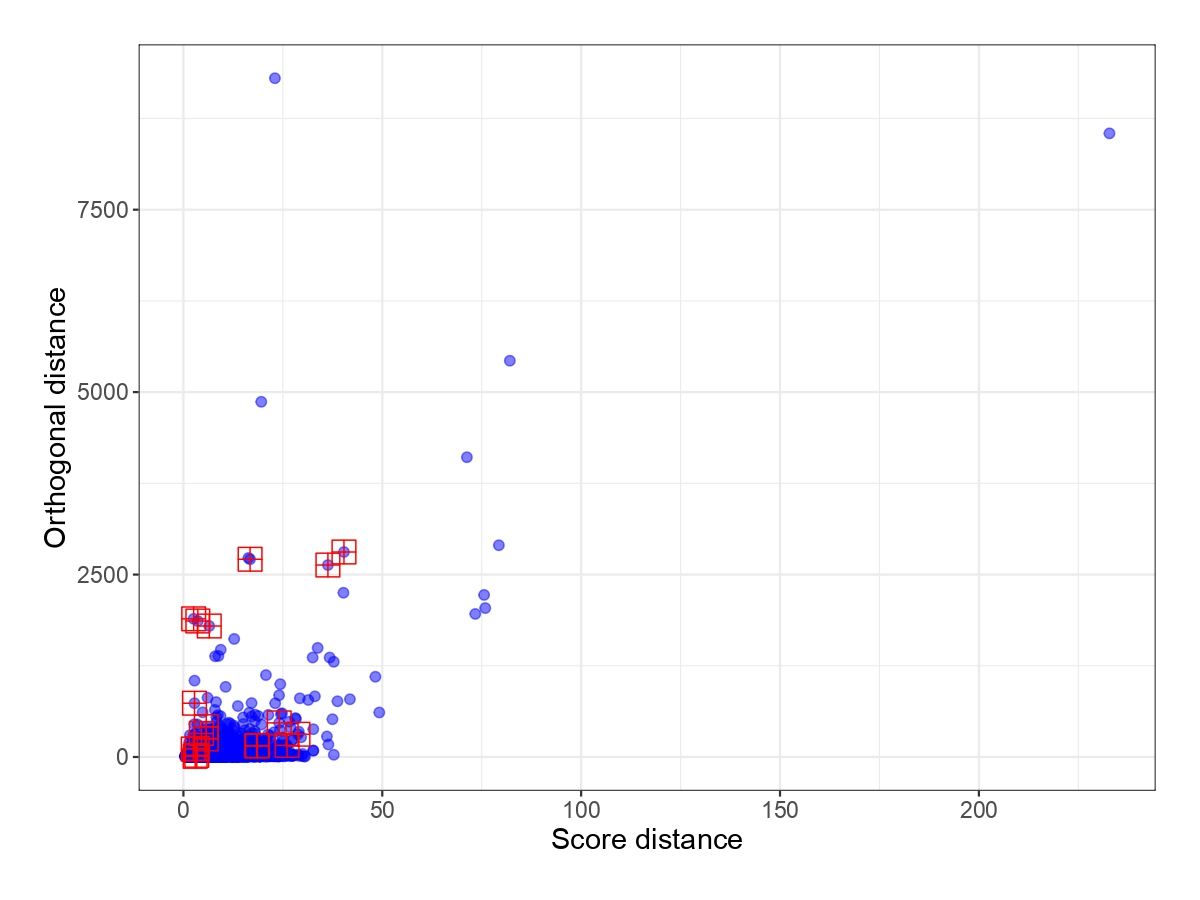
\includegraphics[width=\textwidth]{figures/rpcadpd/CCard-GMed.jpg}
        {\tiny (b) GMedian}
        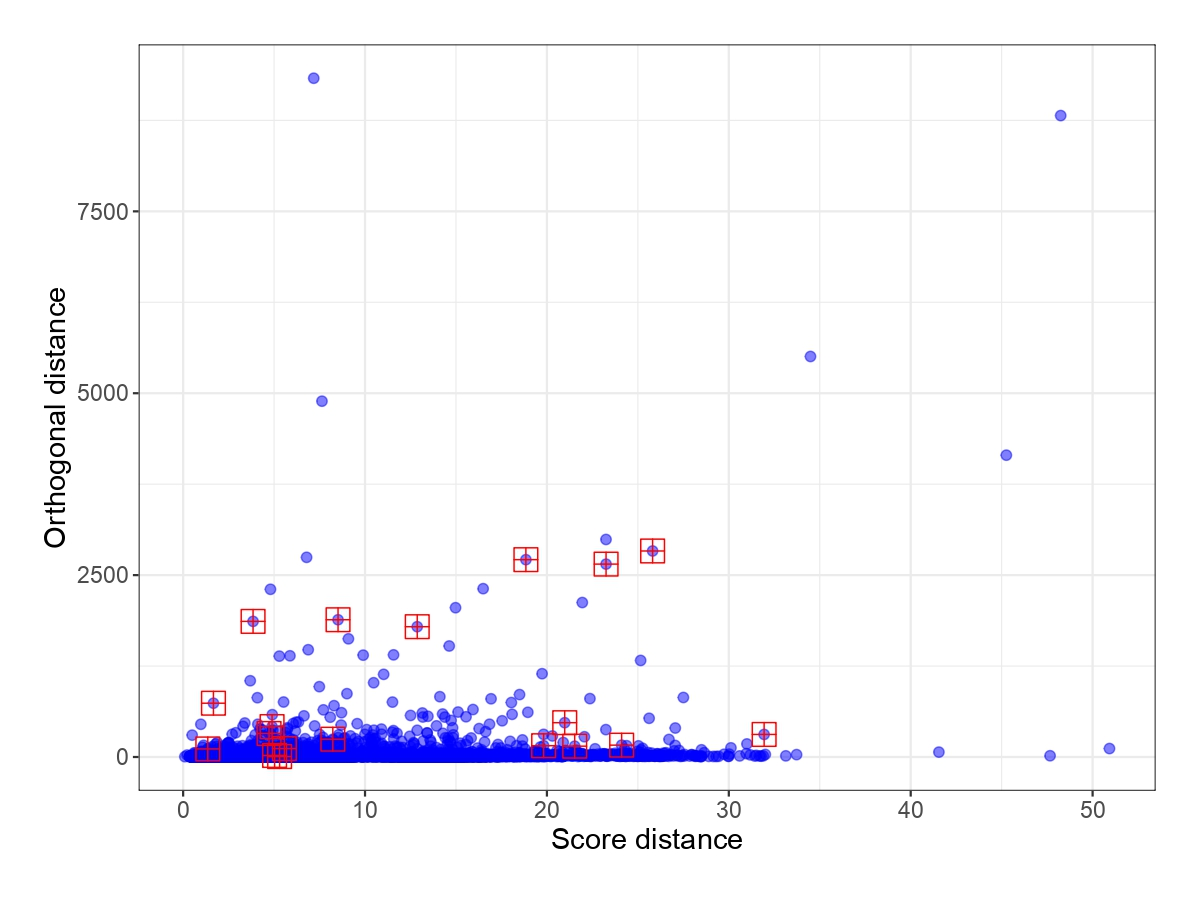
\includegraphics[width=\textwidth]{figures/rpcadpd/CCard-ROBPCA.jpg}
        {\tiny (d) ROBPCA}
    }
\end{columns}
\end{frame}


\begin{frame}{Video Surveillance Background Modelling}
    \begin{columns}
        \column{0.3\textwidth}{
            \frame{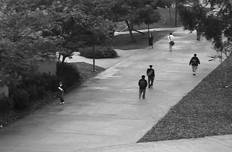
\includegraphics[width = 0.8\textwidth]{figures/rsvd_peds/true_frame170.jpg}}
            {
                \vspace*{-1.85cm}\\
                \hspace{0.25cm}\frame{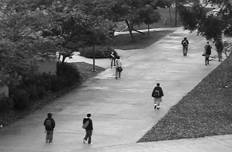
\includegraphics[width = 0.8\textwidth]{figures/rsvd_peds/true_frame1.jpg}}
            }
            {
                \vspace*{-1.9cm}\\
                \hspace{0.5cm}\frame{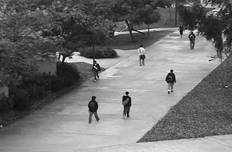
\includegraphics[width = 0.8\textwidth]{figures/rsvd_peds/true_frame107.jpg}}
            }
        }
        \column{2mm}{
            \Large\textbf{=}
        }
        \column{0.3\textwidth}{
            \frame{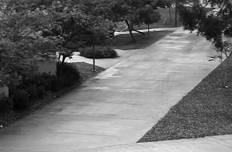
\includegraphics[width = 0.8\textwidth]{figures/rsvd_peds/rsvd_bg_frame170.jpg}}
            {
                \vspace*{-1.85cm}\\
                \hspace{0.25cm}\frame{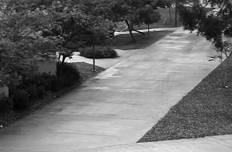
\includegraphics[width = 0.8\textwidth]{figures/rsvd_peds/rsvd_bg_frame1.jpg}}
            }
            {
                \vspace*{-1.9cm}\\
                \hspace{0.5cm}\frame{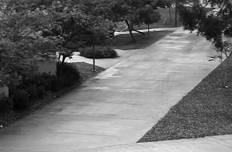
\includegraphics[width = 0.8\textwidth]{figures/rsvd_peds/rsvd_bg_frame107.jpg}}
            }
        }
        \column{2mm}{
            \Large\textbf{+}
        }
        \column{0.3\textwidth}{
            \frame{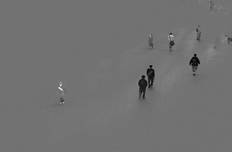
\includegraphics[width = 0.8\textwidth]{figures/rsvd_peds/rsvd_fg_frame170.jpg}}
            {
                \vspace*{-1.85cm}\\
                \hspace{0.25cm}\frame{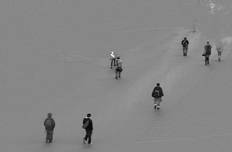
\includegraphics[width = 0.8\textwidth]{figures/rsvd_peds/rsvd_fg_frame1.jpg}}
            }
            {
                \vspace*{-1.9cm}\\
                \hspace{0.5cm}\frame{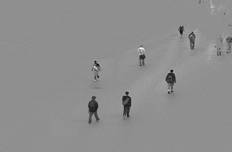
\includegraphics[width = 0.8\textwidth]{figures/rsvd_peds/rsvd_fg_frame107.jpg}}
            }
        }
    \end{columns}
    \begin{equation*}
        \bb{X} (\text{Video}) = \bb{L} (\text{Background}) + \bb{E} (\text{Foreground})    
    \end{equation*}
    
    Following are seconds elapsed per frame for a $640 \times 480$ video.
    \begin{enumerate}
        \item Best existing robust SVD method (\textcolor{blue}{Zhang et al., 2013}) - 312.26
        \item Popular video surveillance method using Robust PCA (\textcolor{blue}{Candes et al., 2011}) - 136.41
        \item Go Decomposition (\textcolor{blue}{Zhou and Tao, 2017}) - 12.06
        \item rPCAdpd (ours) - 2.86
    \end{enumerate}
\end{frame}

\begin{frame}{University of Houston Camera Tampering Dataset}
    \begin{columns}
        \column{0.2\textwidth}{
            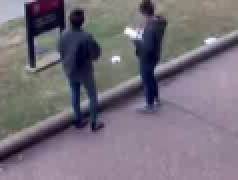
\includegraphics[width = \textwidth]{figures/rsvd_uhctd/true_frame5.jpg}
            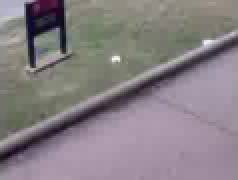
\includegraphics[width = \textwidth]{figures/rsvd_uhctd/true_frame50.jpg}
            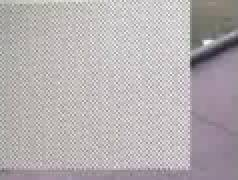
\includegraphics[width = \textwidth]{figures/rsvd_uhctd/true_frame75.jpg}\\
            {\centering Truth}
        }
        \column{0.2\textwidth}{
            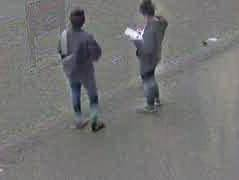
\includegraphics[width = \textwidth]{figures/rsvd_uhctd/OPfg_frame5.jpg}
            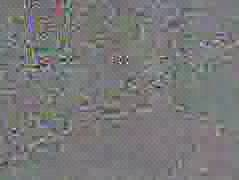
\includegraphics[width = \textwidth]{figures/rsvd_uhctd/OPfg_frame50.jpg}
            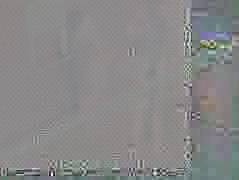
\includegraphics[width = \textwidth]{figures/rsvd_uhctd/OPfg_frame75.jpg}\\
            {\centering OP}
        }
        \column{0.2\textwidth}{
            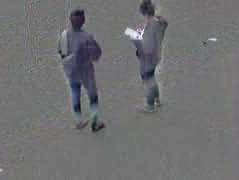
\includegraphics[width = \textwidth]{figures/rsvd_uhctd/ALMfg_frame5.jpg}
            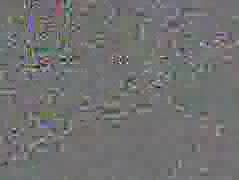
\includegraphics[width = \textwidth]{figures/rsvd_uhctd/ALMfg_frame50.jpg}
            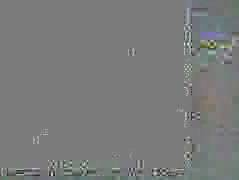
\includegraphics[width = \textwidth]{figures/rsvd_uhctd/ALMfg_frame75.jpg}\\
            {\centering ADMM}
        }
        \column{0.2\textwidth}{
            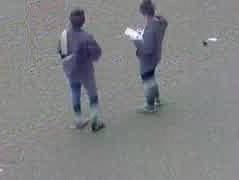
\includegraphics[width = \textwidth]{figures/rsvd_uhctd/GoDecfg_frame5.jpg}
            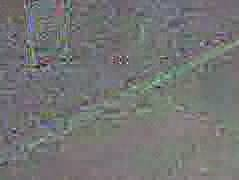
\includegraphics[width = \textwidth]{figures/rsvd_uhctd/GoDecfg_frame50.jpg}
            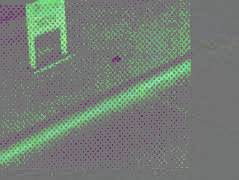
\includegraphics[width = \textwidth]{figures/rsvd_uhctd/GoDecfg_frame75.jpg}\\
            {\centering GoDec}
        }
        \column{0.2\textwidth}{
            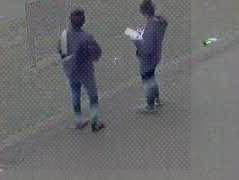
\includegraphics[width = \textwidth]{figures/rsvd_uhctd/rsvddpdfg_frame5.jpg}
            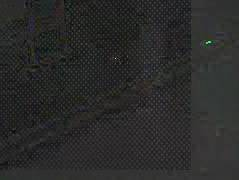
\includegraphics[width = \textwidth]{figures/rsvd_uhctd/rsvddpdfg_frame50.jpg}
            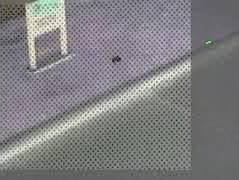
\includegraphics[width = \textwidth]{figures/rsvd_uhctd/rsvddpdfg_frame75.jpg}\\
            {\centering rSVDdpd}
        }
    \end{columns}
\end{frame}


\begin{frame}[shrink=20]
\frametitle{References}
    \begin{thebibliography}{9}
        \bibitem{roy2023pca} Roy, Subhrajyoty, Ayanendranath Basu, and Abhik Ghosh. Robust Principal Component Analysis Using Density Power Divergence. \emph{Journal of Machine Learning Research} 25, no. 324 (2024): 1–40. http://jmlr.org/papers/v25/23-1096.html.
        \bibitem{roy2024video} Roy, Subhrajyoty, Abhik Ghosh. \& Ayanendranath Basu. Robust singular value decomposition with application to video surveillance background modelling. Stat Comput 34, 178 (2024). https://doi.org/10.1007/s11222-024-10493-7.
        \bibitem{roy2023breakdown} Roy, Subhrajyoty, Abir Sarkar, Abhik Ghosh \& Ayanendranath Basu. "Breakdown Point Analysis of the Minimum S-Divergence Estimator." arXiv preprint arXiv:2304.07466 (2023). - \textit{in review}.
        \bibitem{baseetal} Basu, Ayanendranath, et al. "Robust and efficient estimation by minimising a density power divergence." Biometrika 85.3 (1998): 549-559.
        \bibitem{ghoshbasu} Ghosh, Abhik, and Ayanendranath Basu. "Robust estimation for independent non-homogeneous observations using density power divergence with applications to linear regression." (2013): 2420-2456.
        % \bibitem{roy2024breakdown} Roy, Subhrajyoty, Supratik Basu, Abhik Ghosh \& Ayanendranath Basu. "Characterization of Generalized Alpha-Beta Divergence and its Associated Properties." - \textit{in preparation}.
        % \bibitem{roy2024rank} Roy, Subhrajyoty, Abhik Ghosh \& Ayanendranath Basu. "Divergence Information Criterion for Robust Rank Selection" - \textit{in preparation}.
    \end{thebibliography}
\end{frame}

% \begin{frame}[shrink=20]
% \frametitle{Additional References}
%     \begin{thebibliography}{9}
%         \bibitem{dic} Karagrigoriou, Alex, and Takis Papaioannou. "On measures of information and divergence and model selection criteria." Statistical Models and Methods for Biomedical and Technical Systems (2008): 503-518.
%         \bibitem{shabalin} Shabalin, Andrey A., and Andrew B. Nobel. "Reconstruction of a low-rank matrix in the presence of Gaussian noise." Journal of Multivariate Analysis 118 (2013): 67-76.
%         \bibitem{baing} Bai, Jushan, and Serena Ng. "Determining the number of factors in approximate factor models." Econometrica 70.1 (2002): 191-221.
%         \bibitem{owen} Owen, Art B., and Patrick O. Perry. "Bi-cross-validation of the SVD and the nonnegative matrix factorization." (2009): 564-594.
%         \bibitem{kurata} Kurata, Sumito. "On robustness of model selection criteria based on divergence measures: Generalizations of BHHJ divergence-based method and comparison." Communications in Statistics-Theory and Methods 53.10 (2024): 3499-3516.
%     \end{thebibliography}
% \end{frame}


{\setbeamercolor{palette primary}{fg=ag-blue, bg=ag-beige}
\begin{frame}[standout]
  Thank you! \\
  Questions?
\end{frame}
}







\end{document}
